\chapter{PROJECT IMPLEMENTATION\label{ch:PROJECT IMPLEMENTATION}}
\section{ Flow Diagram }
\begin{figure}[!h]
\begin{center}

\tikzstyle{decision} = [diamond, draw, fill=blue!20, 
    text width=4em, text badly centered, node distance=3cm, inner sep=0pt]
\tikzstyle{block} = [rectangle, draw, fill=blue!20, 
    text width=6em, text centered, rounded corners, minimum height=4em]
\tikzstyle{line} = [draw, -latex']
\tikzstyle{cloud} = [draw, ellipse,fill=red!20, node distance=3cm,
    minimum height=2em]

\begin{tikzpicture}[node distance = 4cm, auto]
    % Place nodes
      
    
     \node [block] (node1) {Kinect Input};
     
     \node [block,right of=node1] (node2) {Segmentation};
     
     \node [block,right of=node2] (node3) {Skeletonization};
     
     \node [block,below of=node3] (node4) {Feature \\ Extraction};
     
     \node [block,below of=node2] (node5) {Training \\  the Model};
     
     \node [block,  below of=node1] (node6) {Test a Sign};
     
    % Draw edges
  
    \path [line] (node1) |- (node2);
    
    \path [line] (node2) |- (node3);
    
    \path [line] (node3) -- (node4);
    
    \path [line] (node4) -- (node5);
    
    \path [line] (node5) -- (node6);
    %\path [line] (node5) |- node {ceja} (node6);
    
\end{tikzpicture}
    
\end{center}
\end{figure}

\section{Implementation}
We take input from Kinect using the python library pykinect. We capture the depth frame from the event handler depth frame. This depth frame tells us the different to the object in each pixel. This distance is a 16-bit value out of which one bit is redundant and 3 bits are for player index. So each distance is a 12-bit value. 
\hfill \break
This 12-bit frame is then normalized to 8-bits by bit-by-bit shifting. This 8 bit frame can be seen as an 8-bit image of gray scale. In which the nearer objects are darker than the far objects. So objects at minimum distance would be the darkest.

\begin{figure}[!htb]
	\begin{center}
		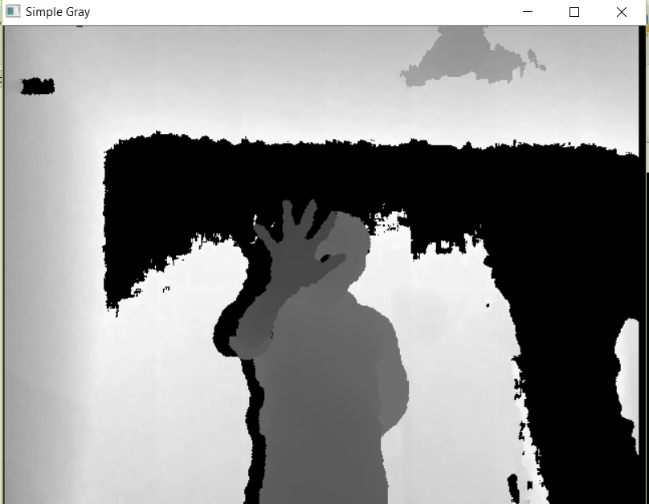
\includegraphics[height=6cm,width=8cm]{ThesisFigs/GrayImage}
		\caption{Gray Image Formation}\label{fig:GrayImage}
	\end{center}
\end{figure}
Note: Any object beyond the range of the Kinect’s optimum range is the darkest.
\hfill \break
Obtained 8-bit gray image is then segmented based on the minimum distance objects from the Kinect. Keep in mind that our project bears a constraint that the signing hand is the only object that is at the minimum distance from the Kinect. So by segmentation based on the minimum distance we get the hand region and using it as a threshold to binary image we will get a binary image with the only signing hand.
\begin{figure}[!htb]
	\begin{center}
		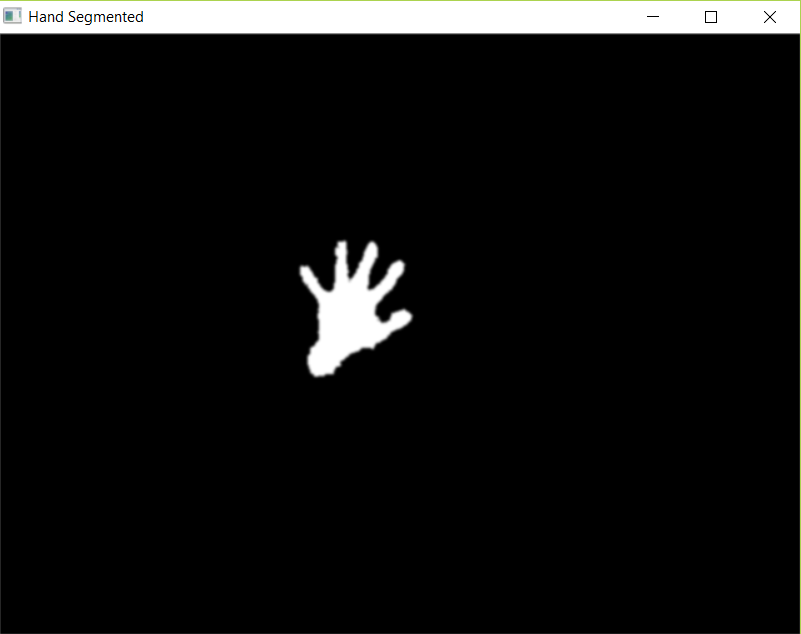
\includegraphics[height=6cm,width=8cm]{ThesisFigs/segmentedImage}
		\caption{Segmented Image}\label{fig:segmentedImage}
	\end{center}
\end{figure}
A segmented image of the above shown gray image is shown.
\hfill \break
We then need to identify all the fingers and the center of the so that these points could be used to generate the feature vectors. For that, we first find the contours (boundary) of the hand. We also find the convex hull in the of the hand shape. Now try and find the points that are common to both the convex hull and the contour of the hand. Both the Convex hull and contours are extracted using OpenCV python. These are the points to be identified as finger tips and corners of the hand. Finger are identified and now these can be used to extract features.
\begin{figure}[!htb]
	\begin{center}
		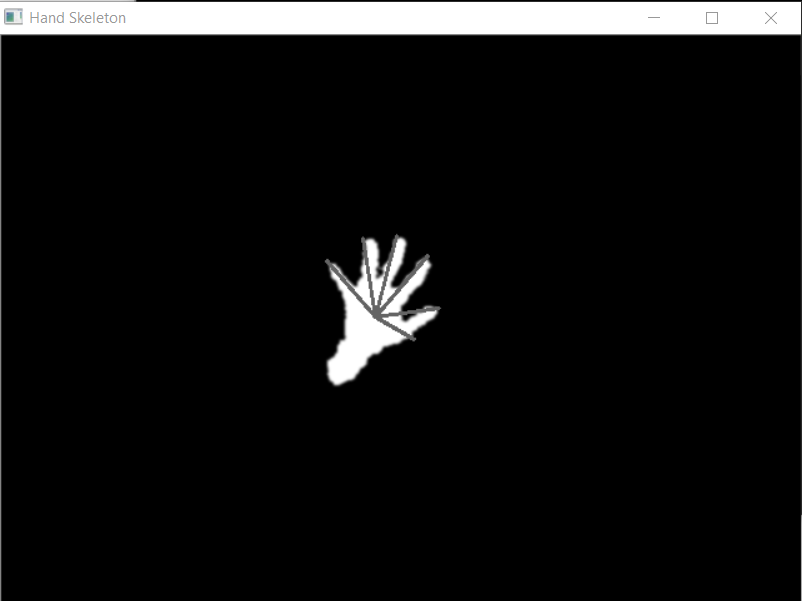
\includegraphics[height=6cm,width=8cm]{ThesisFigs/skeletonImage}
		\caption{Skeleton Image}\label{fig:skeletonImage}
	\end{center}
\end{figure}
Now we find the sum of x-coordinates and also the sum of y-coordinate of all the white pixels (hand-region). Now we divide both x-sum and y-sum by the total number of hand pixels. The obtained point i.e. (x, y) pair is the centroid of the hand.
\hfill \break
Knowing all the main points of the hand region in the frame, we now extract features from the frame to make a feature vector. There are following four main features used:

\begin{itemize}


   \item[•] \textbf {	Consecutive fingers gap :  \\}
  We take the gap of the two consecutive fingers (our choice whether counting from left to right or right to left). This gap      is calculated in the following way:
Say the two fingertips were ‘A’ and ‘B’ points.


\begin{align}
&\sqrt{ [( A.x - B.x )^2 + ( A.y - B.y )^2]} = Distance value (number of pixels)
\end{align}
\item[•] \textbf { Angles of the defects : \\}
  By using the convexity defects (extracted by convex hull and contour of the hand), we get to find the deepest point of the defect which is the considered to be the joint between the two fingers. Now for two consecutive finger tips ‘A’ and ‘B’, we form two vector:
  \begin{enumerate}
  \item From the fingertip ‘A’ to the middle joint of ‘A’ and ‘B’. 
  \item From the fingertip ‘B’ to the middle joint of ‘A’ and ‘B’.
  \end{enumerate}
  Now for the two tips ‘A’ and ‘B’, we get vectors say ‘a’ and ‘b’. Now we apply the following formula.
\begin{equation}
a.b=|a|.|b|cos\theta
\end{equation}
   
From here, if we find the magnitude of ‘a’ and ‘b’ using the distance formula from point ‘A’ to joint and point ‘B’ to joint. And finally, we get angle from the above formula. Now we do that for every defect and use these angles in the feature vector.
 \item[•] \textbf { Area of the hand  : \\}
Area of the hand is number of pixel in the hand region in the respective frame. 
 \item[•] \textbf {Normal distance to convex hull : \\}
Normal distance from each of the joint to the convex hull. The distance is calculate for number of unit pixel and using the simple distance formula.
\end{itemize}

We concatenate all these triplets and area of the hand to form the feature record for the frame. We do that for all the frames and then take them record by record and make a whole file where each record represents a frame in the video.
\\
We combine all these videos of signs and then place all same signs in the same directory and same for all the other classes. As presented in the previous portion (4.3), we pad each video to the length of the maximum size video so that each instance be of the same size and be feasible to train. For padding purpose, we use the Keras python. \\
As all the dataset is in its final form so let’s move in to build the machine learning model for the prediction of signs. A random forest was trained on this dataset with 50 number of trees each of depth 24. Class label was assigned based on majority votes of the tree. Dataset is partitioned to two sets of 75\% part of the whole dataset for training purpose and the rest 25\% part of the dataset for evaluation of the model. Sklearn in python is used to build the model.\\
The interface is built in tkinter python. It contains a window that shows the frame coming right from Kinect. Another field that present you with the label of sign being performed in front of the Kinect. There are also two more buttons labelled as ‘start’ and ‘Predict’. ‘Start’ serves the purpose to allow all the users perform the sign in front of the Kinect. And ‘Predict’ button can be used to terminate the sign duration. As the signer is done with his sign (presses the ‘predict’ button), the sign would be converted into the feature vector and evaluated against the model. In the result of evaluation, a label corresponding to the sign is extracted. This would be presented as the label (textual meaning of sign in Urdu) of the sign performed on the interface screen. \\
For prediction purpose, Random forest is used to classify the signs into sentences. Random forest is a simple but elegant ensemble machine learning technique. It is an ensemble of multiple simple machine learning classifier known as decision trees. It tries to predict class for the sign using different architecture trees i.e. different splits and bootstrapping on the train set. Then takes votes from these trees. And provides the results with majority votes.
As far as Decision trees are concerned, these are simple trees with each node of the tree is a split criteria for a feature. Splits are chosen based on maximum information gain and minimum entropy. And at the leaf there is the class label. An instance when parsed through this tree satisfying different split reaches to its class label. 

\clearpage
\section{Baseline Results}
As discussed and explained in the chapter-4, the complexity and noise of the dataset is huge. Moreover, to make it feasible, we padded the dataset; this also introduces some noise and bias in the dataset. Due to all those reasons, each frame carries some noise with itself and then later this noise convolves with noise of the whole video instance. Presence of all these noises in our dataset leads to a weak model. So the results (predictions) from this model are not fully reliable.\\

The accuracy achieved is 83\% as observed on the 25\% test dataset. Moreover, F1 measure is 0.83.
The prediction time taken by a system of following specification:

\begin{enumerate}
	\item[•]Intel Core i5 processor
	\item[•]8GB RAM
	\item[•]No GPU used
\end{enumerate}

Is 0.446 seconds approximately.
Note that these results are considered as running the system in offline mode i.e. not from the interface. While using the interface accuracy drops because of the frame closing and getting latency introduced by the operations of interface.
\clearpage

\section{Results}
The results are obtained using 10-cross-folds. The simple split across the dataset is 90\% for train and 10\% for test for each fold. Accuracy and F1 score are reliable and significant.\\


\textbf{Results using Random Forest classifiers}
\hfil \break
Results for all folds while using the Random Forest model are shown in Table \ref{randomforest}:

\begin{table}[h]
	\begin{adjustbox}{max width=\textwidth}
		\begin{tabular}{ |p{1.7cm}|c|c|c|c|c|c|c|c|c|c|} 
			\hline
			&  Fold-1 &  Fold-2 &  Fold-3&  Fold-4&  Fold-5&  Fold-6 &  Fold-7	 &  Fold-8&  Fold-9 &  Fold-10     \\ 
			\hline
			Accuracy &  91.667   &  91.667   &  91.667   &  83.333  &  58.333  &  83.333   &  75.0	 &  83.333  &  75.0    &  100.0 \\ 
			\hline
			F1-Score &  0.9144   &  0.9142 &  0.9142&  0.8035&  0.5761&  0.8309     &  0.7416	 &  0.8309&  0.7321 &  1.0 \\ 
			\hline
		\end{tabular}
	\end{adjustbox}
	\caption{Results using Random Forest classifiers\label{randomforest}}
\end{table}

 

The accumulated and finalized results obtained the above given technique and prediction using Random Forest are:

 Cumulative Accuracy of the dataset:	\quad\quad	0.825 (82.5\%) \\
Cumulative F1 Score of the dataset:	\quad\quad	0.83 \\
Entropy and Gini both were used as a splitting criterion and in the test many experiments were run using different number of trees as shown in the figure 5.4 below.
\begin{figure}[!htb]
	\begin{center}
		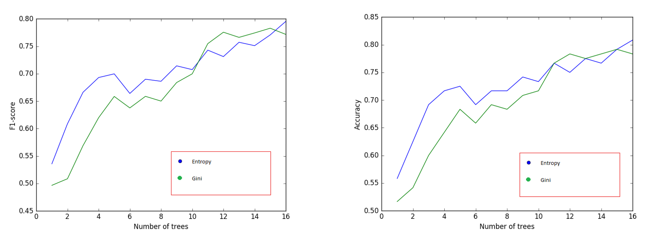
\includegraphics[height=6cm,width=14cm]{ThesisFigs/randomforestgraph}
		\caption{Random Forest Result Graph}\label{fig:randomforestgraph}
	\end{center}
\end{figure}


\clearpage

\textbf{ Alternative Results using SVM classifiers}
\hfil \break
Results for all folds while using the SVM model are shown in Table \ref{svm}:

\begin{table}[h]
	
\begin{adjustbox}{max width=\textwidth}
	\begin{tabular}{ |p{1.7cm}|c|c|c|c|c|c|c|c|c|c|} 
		\hline
		&  Fold-1 &  Fold-2 &  Fold-3&  Fold-4&  Fold-5&  Fold-6 &  Fold-7	 &  Fold-8&  Fold-9 &  Fold-10     \\ 
		\hline
		Accuracy &  100    &  83.333   &  66.6666   &  75  &  50  &  58.333  &  41.666	 &  66.6666  &  75.0    &  100.0 \\ 
		\hline
		F1-Score & 1.0 &	0.8333 &	0.675 &	0.7428 &	0.5	& 0.5863 &	0.3653	& 0.675	& 0.7321 &	1.0 \\ 
		\hline
	\end{tabular}
\end{adjustbox}
	\caption{Results using SVM classifiers\label{svm}}
\end{table}


The accumulated and finalized results obtained the above given technique and prediction using SVM are,

  Cumulative Accuracy of the dataset:	\quad\quad	0.71 (71\%) \\
 Cumulative F1 Score of the dataset:	\quad\quad	0.72 \\

Experiments were run using different degrees of the hyperbola separating the classes. Results are shown in diagram. 
\begin{figure}[!htb]
	\begin{center}
		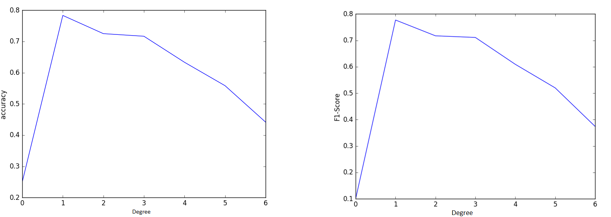
\includegraphics[height=5cm,width=14cm]{ThesisFigs/svmgraph}
		\caption{SVM Result Graph}\label{fig:svmgraph}
	\end{center}
\end{figure}




\textbf{	Alternative Results using Decision Tree classifiers}

\hfill \break Cumulative Accuracy of the dataset:	\quad\quad	0.53 (53\%) \\
  Cumulative F1 Score of the dataset:	\quad\quad	0.55 

Many splitting criterion used are entropy and gini with ranging the depth of tree. Results are shown by fig below. 
\clearpage
\begin{figure}[!htb]
	\begin{center}
		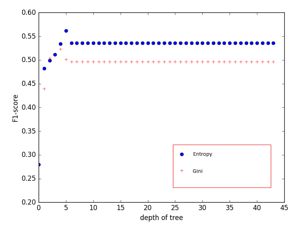
\includegraphics[height=7cm,width=12cm]{ThesisFigs/decisiontreegraph}
		\caption{Decision Tree Result Graph}\label{fig:decisiontreegraph}
	\end{center}
\end{figure}

\textbf{Alternative Results using Naïve Bayes classifiers}
\hfil \break
We also used Naïve Bayes to serve the purpose or build the model. Naïve Bayes worked also fairly well as shown by the following results.

Results for all folds while using the  Naïve Bayes model are shown in Table \ref{naviebayes}:
\begin{table}[h]
	
\begin{adjustbox}{max width=\textwidth}
	\begin{tabular}{ |p{1.7cm}|c|c|c|c|c|c|c|c|c|c|} 
		\hline
		&  Fold-1 &  Fold-2 &  Fold-3&  Fold-4&  Fold-5&  Fold-6 &  Fold-7	 &  Fold-8&  Fold-9 &  Fold-10     \\ 
		\hline
		Accuracy &  50  &	66.666	& 50	& 50	& 25	& 25	& 25	& 41.666	& 75.0	& 58.333\\ 
		\hline
		F1-Score & 0.502 &	0.675	& 0.521 &	0.475 &	0.182	& 171	& 0.214	& 0.375	& 0.555	& 0.497 \\ 
		\hline
	\end{tabular}
\end{adjustbox}

	\caption{Results using  Naïve Bayes classifiers\label{naviebayes}}
\end{table}

\hfil \break
 Cumulative Accuracy of the dataset:	\quad\quad	0.45 (45\%) \\
Cumulative F1 Score of the dataset:	\quad\quad	0.41 \\




\section{Alternative flows and approaches followed}
We tried many flows and strategies but at some point they collapsed or during the feasibility study, they were found to be not compatible with the problem statement. Following are the strategies as listed below.

\begin{enumerate}
	\item \textbf{ RGB and Depth-image overlap for segmentation }
In the starting few frames user is asked to keep his hands in the front of his body and at minimum distance from Kinect. Now take 'AND' of these pixels of binary segmented image with the pixels of the RGB frame to extract the hand region. And now find the bounding box of this hand region in the RGB frame. Extract this region and find its HOG features and append these HOG features from all frames of the video to make feature vector of the sign video.

\item[•] \textbf{Problems with the approach}
\begin{enumerate}
\item The depth frame is zoomed in as compared to the RGB frame. When over-lapping these region would also include some noise of the surrounding.
\item[•]To compute HOG feature, Image must be in the 8 or 16 bit-depth. So to do that, we have to convert each frame to Gray first and then compute HOG. Which takes quite much time; we may lose some key frames. This would take much time and may not allow us to predict in real time for a much larger dataset.
\item HOG features approach would be redundant because for this approach; an instance feature vector would be very huge.
\item[•]For Each frame; the segmented region would be different; we will have to pad the HOG frame to make the size of all frame equal.
\end{enumerate}


\item \textbf{Only RGB hand-tracking and feature Extraction\\}
We had done the hand tracking; our algorithm was tracking the hand with always changing hand shape for each successive frame. Tracking was Real time. Tracking was done using Dlib module that uses localized histograms to get features from a frame and then use these features to track the hand in the successive frames. HOG features were also extracted by converting each frame to gray.
\item[•] \textbf{Problems with the approach}
\begin{enumerate}
\item[•]The Kinect RGB camera is quite noisy. So the hand region that was observed by the specified region from first frames was itself noisy. So while defining the intensity range it would have considered the noise but that was handles by using only the region in the range of standard deviation. But then it starting also segmenting the face and neck region of intensity values. Same were the problems with segmentation based on HSV (Hue, Saturation and Lightness).
\item[•]Region filling in this region was a hectic and noisy job to do.
\item[•]After even segmentation, we were to use some features like HOG or SURF which were redundant in larger and bigger datasets.
\item[•]No significance to use the Kinect Device, if we are to use only the RGB frame.
\end{enumerate}

\item \textbf{Hu-Moments and Zu-Moments \\}
Hu- moments and Zu-Moment are state-of-the-art features to predict static objects and to check whether an object differs from others or not. They are rotation, position and scale invariant features that is why used in many of the applications. We did not extracted these from our frames because we found it these not worthy enough to serve the purpose in this project purpose.
\item[•] \textbf{Problems with this approach}
\begin{enumerate}
\item[•]In the sign language, there is a great significance of hand angle (if hand is rotated or not). As these features are rotation invariant so this would consider a tilted hand and a straight hand as same.
\item[•]These features are significant for only the case, when there are gray values in the region of interest (hand region) but when hand region is identified then it is all the same (flat) intensity values because there is no significant different in the distance from the Kinect Device.
\item[•] No significant results are extracted for sign recognition in the literature.
\end{enumerate}

\item \textbf{LBP features  \\}
LBP features approach finds the local binary patterns as suggested by the names. It goes across the whole image and finds the intensity shifts and captures those in a feature vector for a frame. These features were exempted during the feasibility study phase.
\item[•] \textbf{Problems with this approach}
\begin{enumerate}
\item[•]These features are significant for only the case, when there are gray values in the region of interest (hand region) but when hand region is identified then it is all the same (flat) intensity values because there is no significant different in the distance from the Kinect Device. So no gray region would be in the hand region and hence intensity shifts will remain undetected.
\item[•]No significant results are extracted for sign recognition in the literature.
\end{enumerate}

\item \textbf{SIFT and SURF features  \\}
SIFT as suggested by the name are Scale invariant features which is a plus point in our case. These features apply on RGB and Gray images.
\item[•] \textbf{Problems with the approach}
\begin{enumerate}
\item[•]To compute SURF and SIFT features, Image must be in the 8 or 16 bit-depth. So to do that, we have to convert each frame to Gray first and then compute features. Which takes quite much time; we may lose some key frames. This would take much time and may not allow us to predict in real time for a much larger dataset.
\item[•]SURF and SIFT features approach would be redundant because for this approach; an instance feature vector would be very huge.
\item[•]For Each frame; the segmented region would be different; we will have to pad the SIFT and SURF frame to make the size of all frame equal.
\end{enumerate}

\end{enumerate}
\clearpage
\section{Interface Description}
There are three blocks on the interface. The left block displays the depth stream (transformed to gray image) from the Kinect. The upper right block displays the segmented and skeletonized frame against the frame in the left block at the same time. And lastly, the lower right block contains four item.\\
\begin{itemize}
	\item[•] Text/Label window: Displays the output label against the sign perform in front of the Kinect.
	\item[•]	Start button: Allows user to start performing (recording) the sign.
	\item[•]	End button: Allows the user to stop performing the sign.
	\item[•]	Predict button: Once the sign is performed and saved using the ‘end’ button. User can predict this sign to sentence label using the ‘predict’ button.
\end{itemize}
An interface depiction is given below in which a sign is being performed.

\begin{figure}[!htb]
	\begin{center}
		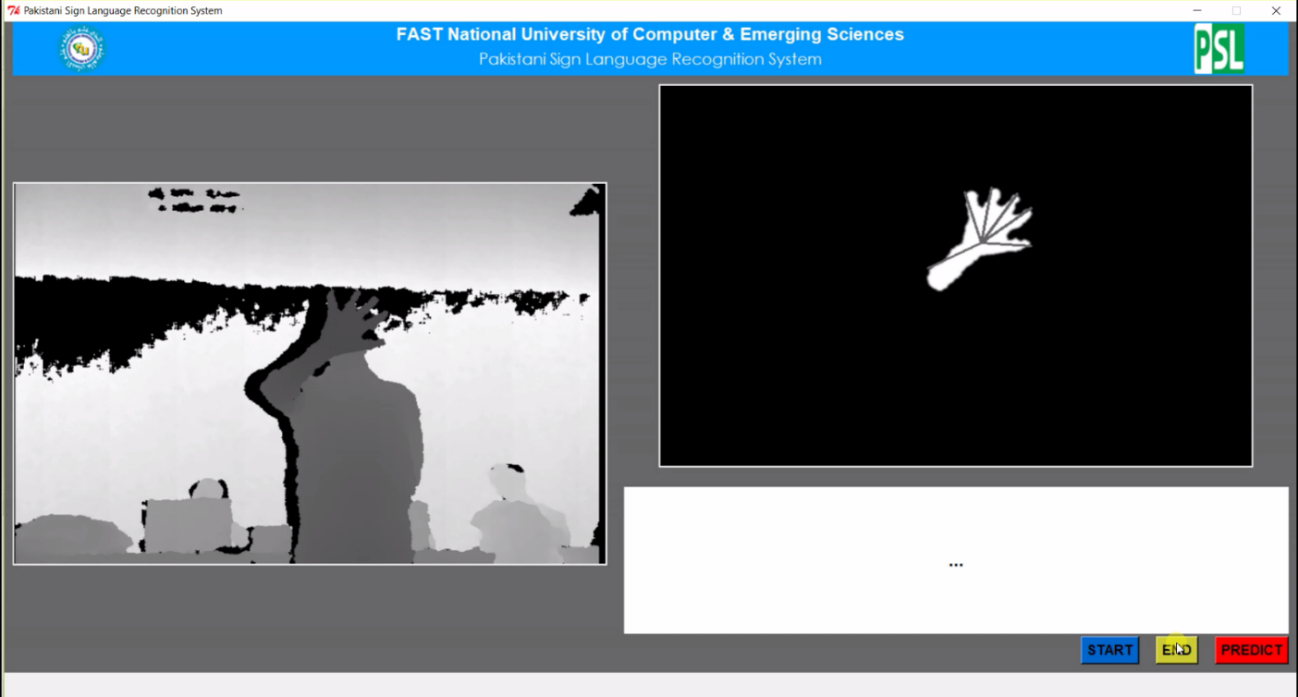
\includegraphics[height=8.5cm,width=12cm]{ThesisFigs/userinterface}
		\caption{User Interface}\label{fig:userinterface}
	\end{center}
\end{figure}
\clearpage
When you press the ‘predict’ button, the label or sentence against the sign is displayed in the Text/Label box as predicted by the model. As depicted by the following image.

\begin{figure}[!htb]
	\begin{center}
		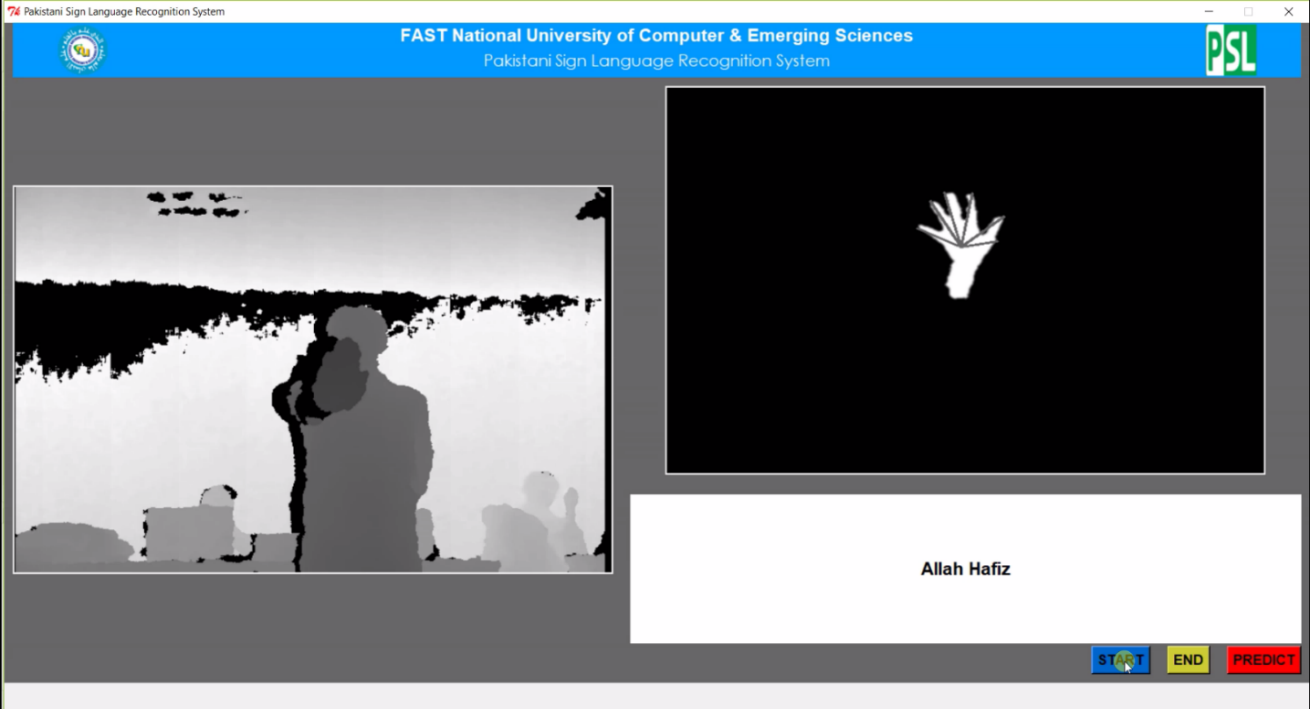
\includegraphics[height=8.5cm,width=12cm]{ThesisFigs/userinterface2}
	
	\end{center}
\end{figure}

